%
% Anlagendesign
%
% @version 1.0
% @author dmayer
% @created 29. Dezember 2015

\setchapterpreamble[o]{%
\dictum[--- \textsc{Charles Eames}]{\Gun Design is the appropriate combination of materials in order to solve a problem. \Gob}}
\renewcommand{\chapterheadstartvskip}{\vspace*{2cm}}

\chapter{Anlagendesign}
\label{chap:anlagendesign}

\renewcommand{\chapterheadstartvskip}{\vspace*{-0.5cm}}

Ziel dieses Kapitel ist es, eine Anlage zur Raumtemperaturregelung für den Betrieb mit Modellprädiktiver Regelung zu konzipieren, zu konkretisieren und im letzten Schritt umzusetzen. Dazu werden zunächst die Anforderungen an die Anlage analysiert und weiterhin die Vorgaben und Rahmenbedingungen zur Anlage von Seiten der Hochschule Karlsruhe spezifiziert und ausgeführt. Daraus wird eine Idee abgeleitet, die anschließend zu einem Konzept weiterentwickelt und in ein konkretes Anlagendesign umgesetzt wird. Dabei werden die einzelnen Anlagenteile und deren Funktionsweisen näher beschrieben und auf die realen Einsatzbedingungen ausgelegt. Abschließend wird die Installation und dabei aufgetretenen Besonderheiten der Anlage beschrieben.

\section{Anforderungen und Konzept Anlage}


\subsection{Analyse der Anforderungen und Rahmenbedingungen}
\label{sec:anforderungen}

Um die Anforderungen an eine Anlage zu bestimmen, die sich sich für die Anwendung mit Modellprädiktiver Regelung eignet, wird zunächst der Zweck und die Einsatzziele der Anlage untersucht und definiert. In Kapitel \ref{sec:motivation} wurde bereits darauf hingewiesen, dass es die Vorgabe von Seiten der Hochschule ist, die Einsatzziele in Einklang mit der großen Anlgae zu bringen und komplementär zu wählen. Daher wurden im Dialog mit den Projektverantwortlichen\footnote{In Person von Herrn \textsc{Adrian Bürger} und \textsc{Markus Bohlayer}} für die Forschung im Bereich solarer Anwendungen an der Hochschule Karlsruhe gemeinsam konkrete Einsatzziele der Anlage erarbeitet. Als Ergebnis wurden die folgenden, konkreten Ziele vereinbart:
 
\begin{itemize}
	\item Die Einarbeitung in die Thematiken Modellbildung, Kommunikation von technischen Systemen und Modellprädiktive Regelung soll durch eine praktisches Anwendung unterstützt werden.
	\item Es soll Know-how im Bereich der Kommunikation von technischen Systemen aufgebaut werden, insbesondere im Umgang mit der Software, der Hardware und zahlreichen Schnittstellen.
	\item Die Anlage soll eine hohe Funktionalität, also möglichst wartungsarm, und eine hohe Robustheit gegenüber Fehlern und Beschädigungen besitzen, da bei der Einarbeitung eine erhöhte Wahrscheinlichkeit der Fehlbedienung besteht und Schäden dadurch vermieden werden sollen.
	\item Es soll ein Vergleich verschiedener Regelungsmethodiken beim Einsatz von Modellprädiktiver Regelung ermöglicht werden.
	\item Außerdem soll ein Vergleich von Ergebnissen bei der Variation von Steuerungsparametern sowie beim Einsatz verschiedener Steuerungs- und Regelungsalgorithmen ermöglicht werden.
	\item Des Weiteren soll die Anlage möglichst flexibel ansteuerbar und erweiterbar sein, damit der Grad der Komplexität anpassbar ist und die Anlage um weitere Funktionen oder Features ergänzt werden kann.
	\item Der temperaturerhöhende Effekt der Sonneneinstrahlung auf die Raumtemperatur soll untersucht werden können.
	\item Im Rahmen der Anwendungsforschung soll der Raum zur Temperaturregelung möglichst nahe an der Realität sein, also Störgrößen beinhalten und nicht ungenutzt beziehungsweise leerstehend sein.
\end{itemize}

Zusammenfassend wurde festgehalten, dass die Anlage als Forschungsumgebung für Entwicklungs-, Test- und Anwendungszwecke von verschiedenen Steuerungen und Regelungen dienen soll.

Weiterhin wurden von Seiten der Hochschule Karlsruhe\footnote{In Person von Frau Professor \textsc{Angelika Altmann-Dieses}, Herrn Professor \textsc{Marco Braun} und Herrn \textsc{Adrian Bürger}} Rahmenbedingungen definiert, die im Folgenden zusammengefasst sind:

\begin{itemize}
	\item Der Raum K004a im K Gebäude der Hochschule Karlsruhe wird zur Installation der Anlage und Einrichtung der Forschungsumgebung zur Verfügung gestellt.
	\item Die Installation der Anlage muss mit minimalem baulichem und finanziellem Aufwand zu realisieren sein.
	\item Für die Kommunikation innerhalb der Anlage soll die Modbus Kommunikationstechnologie mit mindestens zwei verschiedenen übertragungsprotokollen genutzt werden.
	\item Die Modellprädiktive Regelung soll mit Hilfe der Plattform JModelica.org erfolgen.
\end{itemize}

Diese Einsatzziele und Rahmenbedingungen definieren implizit Anforderungen an eine Anlage, welche im Nachfolgenden explizit ausgeführt werden und aus Gründen der übersichtlichkeit die wichtigsten in Tabelle \ref{tab:anforderungen_umgebung} zusammengefasst sind.


\begin{table}[H]
\centering
\small
\renewcommand{\arraystretch}{1.3}
\begin{tabularx}{1\textwidth}{m{0.35\textwidth}m{0.58\textwidth}}

\toprule

\textbf{Einsatzziele \&} & \multirow{2}{\hsize}{\textbf{Anforderungen}} \\ 
\textbf{Rahmenbedingungen} & \\

\cmidrule[0.5pt](r{0.25em}){1-1} 
\cmidrule[0.5pt](l{0.25em}){2-2}

Raum K004a als Umgebung  & \multirow{3}{\hsize}{
\begin{minipage}[t]{0.57\textwidth}
\begin{itemize}[itemsep=0pt,topsep=0pt,leftmargin=5mm]
	\item Die Anpassung der Anlage an K004a.
	\item Die Nutzung bestehender Heizkörper anstatt einer Klimatisierung des Raumes. 
	\item Die Beschränkung auf eine minimale Funktionalität und Anzahl der einzelnen Komponenten. 
\end{itemize}
\end{minipage}
}
 \\
	
\cmidrule[0.1pt](lr{2em}){1-1} 
Minimaler baulicher Aufwand & \\

\cmidrule[0.1pt](lr{2em}){1-1} 
Minimaler finanzieller \newline Aufwand &\\ 



\cmidrule[0.5pt](r{0.25em}){1-1} 
\cmidrule[0.5pt](l{0.25em}){2-2}

\addlinespace[4mm] Modellprädiktive Regelung mit JModelica.org und CasADi \newline & \multirow{3}{\hsize}{
\begin{minipage}[t]{0.57\textwidth}
\begin{itemize}[itemsep=0pt,topsep=0pt,leftmargin=5mm]
\item Die Modellbildung erfolgt in Modelica.
\item Die Ansteuerung und Kommunikation innerhalb der Anlage soll in Python stattfinden	.
\item Die Kommunikation der Anlage erfolgt gemäß den Modbus~RTU und TCP Protokollspezifikationen.
\item Über Modbus~TCP soll die Ansteuerung der Anlage innerhalb des gesamten lokalen Netzwerks möglich sein.
\end{itemize}
\end{minipage}
}  \\

\cmidrule[0.1pt](lr{2em}){1-1}
\addlinespace[4mm] Einsatz der Modbus \newline Kommunikationstechnologie \newline 	& 		\\

\cmidrule[0.1pt](lr{2em}){1-1}
\addlinespace[4mm] Flexible Ansteuerung der Anlage \newline & \\

\cmidrule[0.5pt](r{0.25em}){1-1} 
\cmidrule[0.5pt](l{0.25em}){2-2}

Einarbeitung in die Thematiken:
\begin{minipage}[t]{0.34\textwidth}
\begin{itemize}[itemsep=0pt,topsep=0pt,leftmargin=4mm]
	\item Modellbildung,
	\item Kommunikation technischer \newline Systeme,
	\item und Modellprädiktive \newline Regelung.
\end{itemize}
\end{minipage}
 	& \multirow{2}{\hsize}{
\begin{minipage}[t]{0.57\textwidth}
\begin{itemize}[itemsep=0pt,topsep=0pt,leftmargin=5mm]
	\item Komplexität ist notwendig, darf jedoch nicht zu hoch sein.
	\item Es sind möglichst wenige thematische überschneidungen erwünscht, daher wird eine klare Struktur mit möglichst scharfer Trennung benötigt.
\end{itemize}
\end{minipage}
}  \\

\cmidrule[0.1pt](lr{2em}){1-1} 

Know-how für Kommunikation \newline technischer Systeme 	&		\\

\cmidrule[0.5pt](r{0.25em}){1-1} 
\cmidrule[0.5pt](l{0.25em}){2-2}

Vergleich von Ergebnissen durch:
\begin{minipage}[t]{0.34\textwidth}
\begin{itemize}[itemsep=0pt,topsep=1pt,leftmargin=4mm]
	\item die Variation von \newline Steuerungsparametern,
	\item den Einsatz verschiedener \newline Regelungsmethodiken,
	\item und den Einsatz \newline verschiedener Algorithmen.
\end{itemize}
\end{minipage}

& \multirow{3}{\hsize}{
\begin{minipage}[t]{0.57\textwidth}
\begin{itemize}[itemsep=0pt,topsep=0pt,leftmargin=5mm]
\item Die Reaktion des Systems muss schnell messbar sowie günstig und einfach zu erfassen sein.
\item Der Einsatz von robusten und einfachen Bauteile.
\item Nutzung eines wartungsarmen Systems.
\item Eine einfache, modulare Erweiterbarkeit des Systems für weitere Schritte muss gegeben sein.
\end{itemize}
\end{minipage}
}  \\

\cmidrule[0.1pt](lr{2em}){1-1} 

Hohe Funktionalität und \newline Robustheit & \\

\cmidrule[0.1pt](lr{2em}){1-1} 

Erweiterbarkeit der Anlage
 &  \\

\bottomrule
\end{tabularx}
\caption{Umsetzung der Ziele in Anforderungen der Anlage}
\label{tab:anforderungen_umgebung}
\end{table}

Die grundlegendste Anforderung an die Planung, ist die Anpassung an die Lage und die Gegebenheiten des Raumes K004a, welche in \ref{fig:skizzek004a} skizziert sind. Der Raum befindet auf dem Campus der Hochschule Karlsruhe, an der südwestlichen Ecke des K Gebäudes im Erdgeschoss. Die südliche und westliche Wand teilt sich der Raum mit der Außenumgebung und wird im Folgenden als Außenwand bezeichnet. Die östliche und nördliche Wand sowie die Decke und der Boden des Raumes grenzen an andere Räume im K Gebäude. Außerdem ist in der südlichen Außenwand eine Fensterfront mit Jalousien zur Verschattung eingebaut und direkt darunter ein Heizkörper installiert.

\begin{figure}
\centering
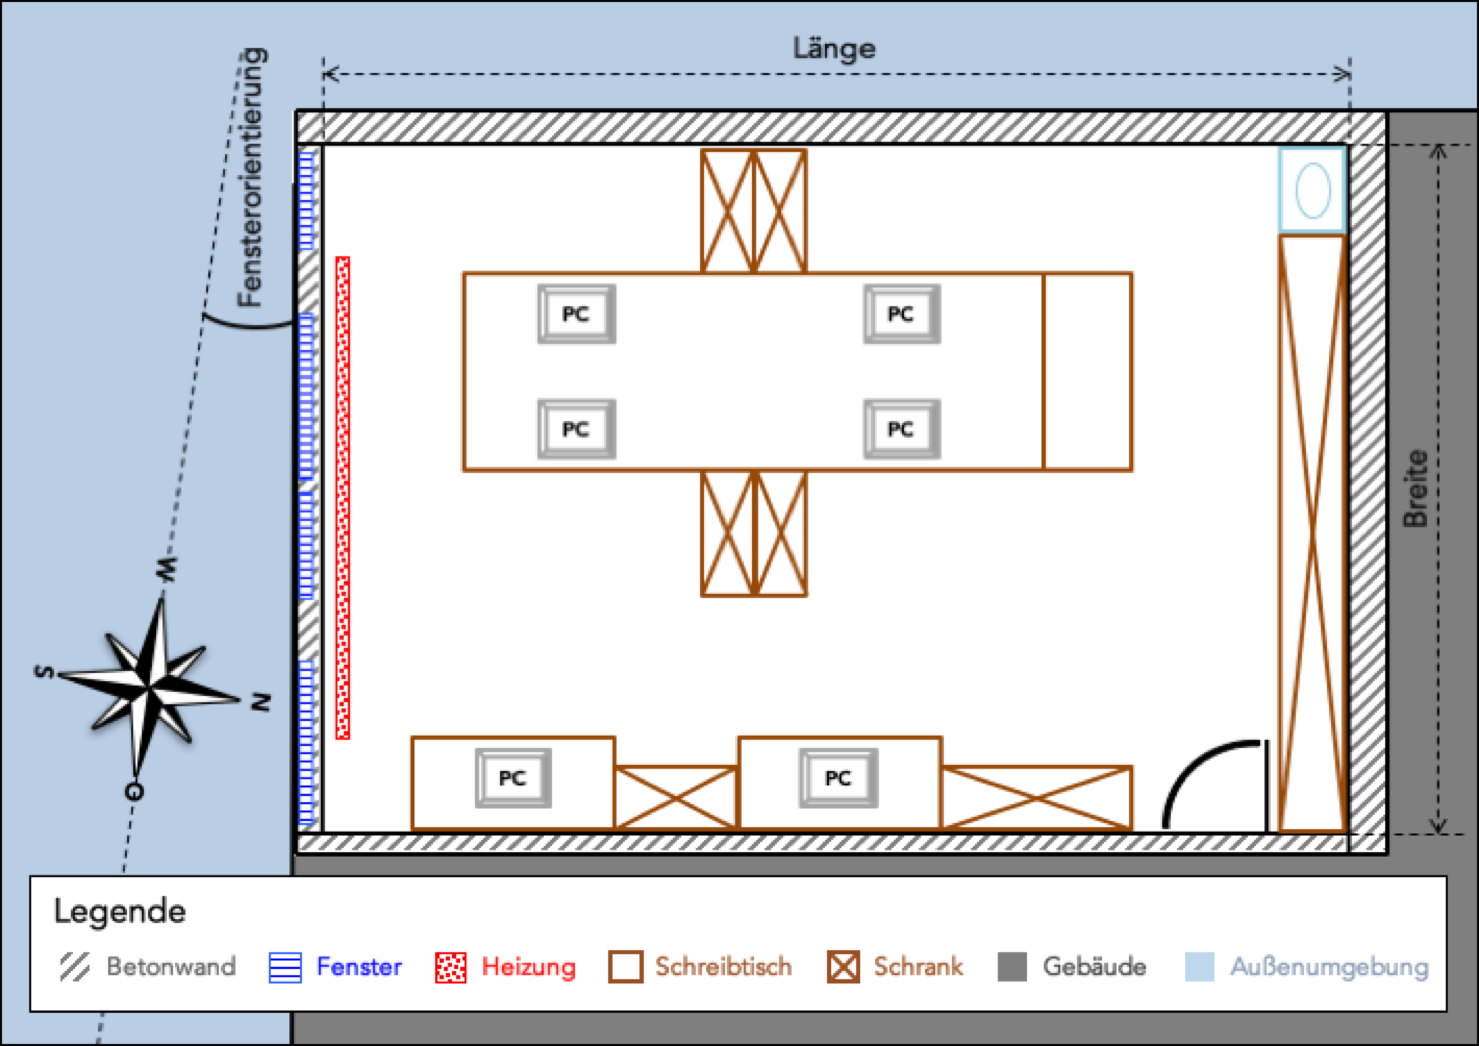
\includegraphics[width=\textwidth]{abbildungen/20160102_k004a}
\caption[Raumskizze K004A vom K Gebäude der Hochschule Karlsruhe -- Technik und Wirtschaft]{Raumskizze K004A vom K Gebäude der Hochschule Karlsruhe -- Technik und Wirtschaft}
\label{fig:skizzek004a}
\end{figure}

Durch die Raumwahl werden bereits zwei wichtige Anforderungen erfüllt, denn durch die Fensterfront kann der Einfluss der Sonneneinstrahlung auf die Raumtemperatur untersucht werden und der bestehende Heizkörper kann in die Anlage integriert werden, um einen minimalen baulichen Aufwand sicherzustellen. Damit wird zunächst eine Klimatisierung zur Temperaturregelung des Raumes ausgeschlossen, weil diese mit einem erheblichen finanziellen und baulichen Aufwand verbunden ist. Um der Forderung nach einer Erweiterbarkeit nachzukommen, wird jedoch die Möglichkeit der Nachrüstung einer Klimatisierung und der Ansteuerung der Jalousien bei der Planung explizit berücksichtigt.

Durch die Nutzung des Raumes als Büro für wissenschaftliche Mitarbeiter befinden sich in K004a sechs Computerarbeitsplätze sowie das typische Büro-Mobiliar, wie in \ref{fig:skizzek004a} abgebildet. Damit wird auch die Anforderung einer anwendungsnahen Umgebung erfüllt und durch die Menschen und Rechner sind verschiedene Störgrößen zu berücksichtigen.

Eine weitere, sehr einschränkende Vorgabe ist es, dass die Modellprädiktive Regelung unter Zuhilfenahme der Plattform \textsc{JModelica.org} erfolgen soll. \textsc{JModelica.org} ist eine kostenlose Open-Source Plattform	 zur Analyse, Simulation und Optimierung von komplexen, dynamischen Systemen, die auf der Modellierungssprache Modelica basiert. Aufbauend auf den mathematischen Modellen physikalischer Systeme in Modelica, lassen sich, dank der Unterstützung der Spracherweiterung Optimica, Optimierungsprobleme durch einfache Konstrukte das Optimierungsintervall, die Kostenfunktion und die Nebenbedingungen einfach formulieren. JModelica.org wird über eine Python Nutzerschnittstelle genutzt und besitzt eine eigene Klasse für die Modellprädiktive Regelung, auch wenn diese bisher noch experimenteller Art ist \cite[S.~1f.]{jmod15}.
Der Compiler kann die Modelle und Optimierungsprobleme in verschiedene Formate übersetzen. Zum einen in direkt ausführbaren C Code, der die Modellgleichungen und Optimierungsparameter enthält, und ein XML Code, der die Meta-Daten des Modells enthält. Zum anderen kann das Modell aber auch in ein \textit{OptimizationProblem} Objekt transferiert werden, welches eine symbolische Repräsentation des Optimierungsproblems ist \cite[S.~12ff.]{jmod15}.

Die \textit{OptimizationProblem} Objekte können anschließend direkt mit den Optimierungswerkzeugen von \textsc{CasADi} bearbeitet und damit zur Lösung des Optimierungsproblems eingesetzt werden. \textsc{CasADi} ist ein Open-Source Softwaretool, das einzelne Bausteine für die numerische Optimierung im Allgemeinen und für die Optimalsteuerung im Speziellen zur Verfügung stellt. Es eignet sich besonders für die gradientenbasierte, numerische Optimierung von nichtlinearen Problemen, aufgrund seiner effizienten Ableitungserzeugung durch die Algorithmische Differentiation und und der Möglichkeit zur Integration von gewöhnlichen Differenzialgleichungen und differential-algebraischer Gleichungen. Die Interaktion mit dem Nutzer soll aus Stabilitätsgründen über die Python Schnittstelle erfolgen \cite[S.~5f.]{casadi}.
Daraus resultieren weitere Anforderungen an das Modell, welche vor Beginn der Modellbildung im Kapitel \ref{chap:modellbildung} erörtert werden.

%Until here fine

Weil die vorgegebene Softwareplattform zur Modellprädiktiven Regelung und deren Komponenten eine allesamt eine Schnittstelle für Python besitzen, soll die Ansteuerung und Kommunikation der gesamten Anlage in Python erfolgen. Python eignet sich hervorragend für diese Aufgabe, da es frei erhältlich und modular aufgebaut ist. Durch die Open-Source Lizenzierung ist es frei nutzbar und bietet sowohl durch die Standardbibliothek als auch durch eine Vielzahl an nutzerentwickelten Bibliotheken, die auch als Pakete bezeichnet werden, unzählige Anwendungsmöglichkeiten, zum Beispiel das pysolar Paket, das im Rahmen der Modellbildung eine Umrechnung der gemessenen Solarstrahlung in die wirkende am Fenster ermöglicht \cite[S.~2f.]{python}.

Der Vorgabe der Modbus Kommunikationsprotokolle für die Kommunikation ist von ebenfalls von großer Relevanz, da die komplementäre Forschungsanlage zur solaren Klimatisierung dasselbe Kommunikationsprotokoll unterstützt und durch die gewonnenen Erkenntnisse eine beschleunigte Inbetriebnahme erfolgen kann. Um das Know-how breit zu fächern, sollen die beiden Modbus RTU und Modbus TCP Protokolle Anwendung finden. Außerdem soll das Kommunikationsnetzwerk aus mehreren Subnetzwerken aufgebaut sein, die durch verschiedene elektrische und mechanische Schnittstellen implementiert werden. Für die Kommunikation über Modbus werden in den Python Paketen pymodbus, minimalmodbus und modbus-tk bereits Bausteine zur Verfügung gestellt.

Die Anlage sollte möglichst wenig Komplexität aufweisen, damit die Einarbeitung in die einzelnen Themengebiete Modellbildung, Kommunikation von technischen Systemen und Modellprädiktive Regelung vereinfacht wird. Dies soll durch eine klare Abgrenzung der Funktionen von verschiedenen Anlagenteilen und durch die Strukturierung sowie den Aufbau der Anlage erreicht werden. %Merker
Im Gegensatz dazu, steht die Forderung nach dem Aufbau von speziellem Know-how bei der Kommunikation technischer Systeme. Um Know-how zu generieren sollen verschiedene Hard- und Software-Schnittstellen kombiniert eingesetzt werden. Allerdings mit einer wachsenden Anzahl von Schnittstellen auch eine Erhöhung der Komplexität einhergeht.
Deshalb muss nach einem Kompromiss zwischen Verständlichkeit und Komplexität gesucht werden, weshalb ein bestimmtes Maß an Komplexität erwünscht ist.


Um das Vergleichen von Ergebnissen zu ermöglichen und weitestgehend zu vereinfachen, sollen die Reaktionen auf Veränderungen schnell stattfinden\footnote{Im Kontext von thermischen Systemen heißt schnell im Minutenbereich} und einfach zu messen sein. Das bedeutet konkret, dass die Anlage und Raumtemperatur zum einen \Gun schnell\Gob eine Reaktion auf Steuerungsimpulse zeigen soll, zum anderen soll die Reaktion einfach, dass heißt ohne großen technischen und monetären Aufwand und möglichst direkt, messbar sein. 
Außerdem sollen eine hohe Funktionalität gegeben sein, dass heißt eine möglichst wartungsarm und Fehlerquellen auszuschließen und damit die wissenschaftliche Arbeit zu erleichtern. Entsprechend wird auch eine Robustheit gegenüber Fehlern gefordert, da bei Testeinsätzen von Steuerungs- und Regelungsalgorithmen sowie bei der Einarbeitung in die Anlage und Themengebete eine erhöhte Gefahr/Wahrscheinlichkeit in Bezug auf das Fehler passieren besteht und diese keinen Schaden an der Anlage verursachen sollen. Deshalb sollen die einzelnen Komponenten der Anlage möglichst einfach aufegbaut sein und ohne technischen Schnickschnack sein, was auch wiederum zur Forderung der minimalen finanziellen Belastung passt.

Da alle bereits genannten Hard- und Softwarekomponenten haben eine Python Schnittstelle besitzen beziehungsweise frei nutzbare Pakete in Python als Schnittstelle zur Verfügung stehen, soll auch die Ansteuerung der gesamten Anlage in Python stattfinden. Damit kann Python als gemeinsamer Nenner für Ansteuerung Anlage und Optimalsteuerung genutzt werden und es kann ein minimaler Rechner dazu genutzt werden, wie z.B. ein Raspberry Pie. Daher wird die gesamte folgende Planung darauf aufbauen, dass sie sich in/aus Python steuern lässt.


\subsection{Idee}

Eine erste, grobe Idee, welche in den folgenden Abschnitten sukzessive an die an die obigen Anforderungen angepasst wird, ist also eine Anlage zur Regelung der Temperatur im Raum, die so minimal wie möglich aufgebaut ist. Konkret gilt es zunächst die Raumtemperatur über Sensoren zu erfassen und diese weiterhin mit Hilfe des Heizkörpers zu steuern. Ein minimaler Aufbau lässt sich in drei Gruppen/Klassen von Anlagenteilen gliedern: Die Sensorik zur Ermittlung des Zustandes im Raum und der Steuergrößen, der Aktorik zur aktiven Beeinflussung des Raumzustandes und einen zentralen logischen Controller, der das Zusammenspiel der einzelnen Anlagenteile und Komponenten koordiniert und die Modellprädiktive Regelung steuert.
Nachdem die Anforderungen konkretisiert und erläutert wurden und die Idee der Anlage klar ist, wird diese nun weiter konkretisiert, entsprechend der drei zuvor gebildeten Gruppen.

Der logische Controller ist die zentrale Komponente der Anlage, da dieser die gesamten Steuerungs- und Kommunikationsaufgaben übernimmt. Dazu nutzt er die Sensorik und Aktorik um sein Ziel der Temperaturregelung zu erreichen und wird genutzt um  Optimalsteuerungspläne berechnet werden müssen wird dazu eine ausreichende Rechenkapazität benötigt. Um diesen Aufgabenumfang abarbeiten zu können und um dem minimalen finanziellen Aufwand genüge zu tragen, wird hierzu zunächst ein freier Rechner der Hochschule Karlsruhe genutzt.

Bei der Temperaturregelung interessiert lediglich die Raumtemperatur, welche als Zustand aufgefasst wird. Daher wird zunächst ein Sensor zur Bestimmung der Raumtemperatur benötigt. Da jedoch die Temperatur innerhalb des Raumes mit hoher Wahrscheinlichkeit nicht homogen ist, werden mehrere Sensoren zur Temperaturmessung benötigt, weshalb mindestens zwei Sensoren benötigt werden.

Für die Erwärmung des Raumes muss gemäß den Anforderungen der Heizkörper innerhalb des Raumes genutzt werden. Um den Heizkörper ansteuern zu können, wird ein Aktor benötigt, der das Ventil am Heizkörper öffnen und schließen kann. 
Durch das ansteuern des Heizkörpers kann die eingebrachte Wärmemenge in den Raum kontrolliert werden, jedoch ist die eingebrachte Wärmemenge des Heizkörpers in den Raum abhängig von verschiedenen Faktoren. Dazu gehören zum einen der Massendurchfluss sowie die Temperatur des Heizwassers am Ein- und Auslass des Heizkörpers, welche der Controller zur Modellprädiktiven Regelung benötigt. Um diese zu erfassen werden also zwei weitere Temperatursensoren und ein Durchflusssensor benötigt.

Dieses Set-Up/Einrichtung ist in \ref{fig:konzept} graphisch dargestellt.

Dieses Konzept bietet langfristig auch die Möglichkeit die Anlage durch eine Klimatisierung zu erweitern, um die Raumtemperatur ganzjährig beziehungsweise in beide Richtungen zu regeln zu können. Außerdem besteht die Möglichkeit in diesem Zuge auch das öffnen und Schließen der Jalousien ebenfalls von der Anlage aus gesteuert werden kann.

Damit steht das Konzept der Anlage und im nächsten Abschnitt kann eine detaillierte Planung der Bauteile, Verdrahtung und Komponenten und Protokolle erfolgen.

\section{Planung und Umsetzung der Anlage}

\subsection{Planung der Anlage}

Wie bereits erwähnt stellt der Rechner das Zentrum der Anlage dar. Deshalb wird darauf aufbauend zunächst die Kommunikationsleitungen und das Netzwerk geplant. Die Kommunikation soll gemäß den Spezifikationen über die Modbus Protokolle RTU und TCP geschehen. Da der Rechner einen Netzwerkanschluss für ein Ethernet besitzt, soll darauf basierend das Netzwerk aufgebaut werden. Für den zusätzlichen Einsatz des Modbus RTU Protokolls wird ein weiteres serielles Netzwerk aufgebaut, dass mit Hilfe eines Gateways an das modbus Ethernet angeschlossen wird. Dieses übernimmt die Aufgabe der übersetzung der Kommunikation zwischen dem Ethernet und dem seriellen Teil des Netzwerks übersetzt.

Die Temperatursensoren sollen als Raumtemperaturfühler ausgeführt werden und an zwei Stellen des Raumes die Temperatur messen. Des Weiteren sollen sie möglichst günstig sein und eines der beiden eingesetzten Modbus Protokolle unterstützen. Die Positionierung ist in Abbildung REFXXXX graphisch dargestellt und erfolgt auf einer raummittig gedachten Achse in nord-südlicher Richtung, jeweils am Ende der Schreibtische. Einer in Richtung der Fenster, der andere gegenüber am Ende der Schreibtische.

Um die Heizung mit den benötigten Sensoren auszustatten, bietet sich ein Wärmemengenzähler an. Dieser integriert die benötigten Sensoren und hat zusätzlich ein Rechenwerk, dass mit einem mit Modbus-Kommunikationsmodul ausgestattet werden kann zum Auslesen der einzelnen Messwerte.

Um den Massenfluss im Heizkörper über das Ventil ansteuern zu können wird ein Stellantrieb benötigt. Dieser kann durch einen Elektromotor oder durch ein thermisches Element angetrieben werden. Die Ansteuerung des Stellantriebs erfolgt üblicherweise durch ein digitales oder analoges Signal, wodurch sich eine weitere Schnittstelle ergibt und ein Modbus-Signalwandler eingesetzt werden kann.

Auf Basis dieser Spezifikationen werden die folgenden zum Einsatz kommenden Bauteile eingesetzt
%&Here we go

\subsection{Temperatursensoren}
Eine kostengünstige und  dingens Möglichkeit, die Raumtemperatur zu erfassen und über eine serielle Modbus RTU Schnittstelle abzufragen bietet der eingesetzte Raumtemperaturmessumformer THERMASGARD RTM1-Modbus von S+S Regeltechnik. Zwei Stück davon kommen in der Ausführung ohne LCD Anzeige zum Einsatz. 
Bei der Installation der Anlage konnten von Seiten der HSKA noch zusätzliche Temperatursensoren zur Verfügung gestellt werden. Diese haben keine Modbusanschluss, können aber über ein Ethernet Lokales Netzwerk über das http Protokoll vom Controller ausgelesen werden. Daher wurden diese in die Anlage integriert und die Anordnung der Anlage verändert wie in REFXXXXXX dargestellt. Die Sensoren werden entlang der westlichen Außenwand und der östlichen Innenwand gleichmäßig verteilt und auf einer Höhe von 2m installiert, um ein gutes Bild der Raumtemp verteilung zu erhalten. Die sechs Sensoren wurden zur Identifizierung gemäß REF XXXXXXXXX bezeichnet

\subsection{Wärmemengenzähler}

Ein mutlifunktionelles und kostengünstiger Wärmemengenzähler ist das MULTICAL 602 Rechenwerk zur Wärmemessung zusammen mit einem impulsgebenden Durchflusssensor sowie einem Temperatursensorpaar. 
Dank seiner hohen Messgenauigkeit registriert der Zähler den genauen Verbrauch über die ganze Lebensdauer des Zählers. Der Zähler ist wartungsfrei, hat eine lange Lebensdauer, und garantiert so- mit minimale jährliche Betriebskosten.
zusammen mit dem Durchflusssensor ULTRAFLOW 54 verwendet. Die Durchflussgrößen decken den Bereich von qp 0,6 m3/h bis qp 1.000 m3/h.
MULTICAL® 602 auszeichnet sich durch die komplette Auswahl von Kommunikationsmodulen und die eingebaute RTC (Echtzeituhr), die es leicht machen, den Zähler in allen Applikationen anzupassen, unabhängig von der Auslesemethode.
Für drahtgebundene Kommunikation kann der Zähler mit Modbus, Datenmodul ausgestattet werden.
Schließlich garantiert MULTICAL® 602 mit ULTRAFLOW® und den genau gepaarten Temperaturfühlern präzise Messergebnisse eben bei minimalen Temperaturunterschieden. Die Langzeitstabilität und Genauigkeit des Durchflusssensors wird nicht von Durchflussgeschwindigkeit, Durchflussstörungen und Verschleiß beeinflusst, was für einer optimalen Betrieb sorgt.

\subsection{Signalwandler und Stellantrieb}

Das EX9024 Analog Out 14bit Modul lässt sich leicht in ein RS485-Netzwerk einbinden. Das Analog Out RS485 Modul hat vier analoge Ausgänge die Spannungen in den Bereichen ±5VDC, ±10VDC, 0~5VAC und 0~10VAC ausgeben können. Das RS485 Analog Out Modul ist für den erweiterten Temperaturbereich ausgelegt.

Thermischer stellantrieb ABNM-LIN, 0-10 Vdc, proportional
Der antrieb ABNM ist ein thermoelektrischer Stellantrieb zum Öffnen und Schließen vonn Ventilen im Bereich Heizungs-, Lüftungs- und Klimatechnik.
Die Regelung erfolgt über ein 0-10 Vdc Signal, das entweder von einem Raumthermostat oder in den meisten Fällen von der zentralen Leittechnik (DDC) bereitgestellt wird. Der Stellantrieb wandelt das 0-10 Vdc Signal in einen proportionalen Stellweg um, der linear oder logarithmisch sein kann.



\subsection{Gateway}
Das Gateway bietet eine einfache und kostengünstige Möglichkeit, um ein serielles Netzwerk in ein Lokales Netzwerk zu integrieren. Dadurch ist es möglich Modbus RTU Geräte von einem Modbus TCP/IP Clienten zu steuern. Zum Einsatz in der Anlage kommt das EX9132C-2-MTCP Gateway von ExpertDAQ, welches übe über zwei serielle Ports verfügt, ein EIA-232 und ein EIA 232/422/485 Port. Die genauen Spezifikationen können dem Datenblatt im Anhang REFXXXXXXXX entnommen werden. Damit kann 

\section{Umsetzung und Installation}


